% Asset ID: AS1TrigonometricRatiosTIKZ-010
% Source: P1-Chp9 p.5
% Related section: Definitions
% Purpose: Cosine as complementary sine
\documentclass[tikz,border=8pt]{standalone}
\usepackage{amsmath}
\usetikzlibrary{angles,quotes,calc,arrows.meta}
\begin{document}
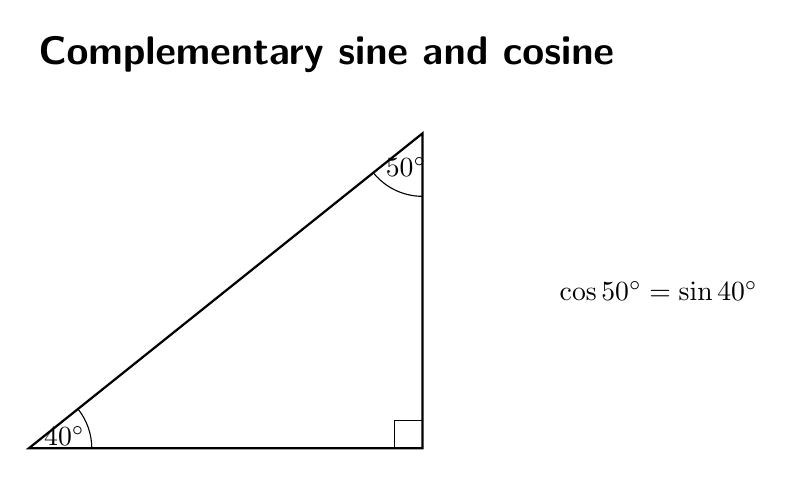
\begin{tikzpicture}[scale=1.0, every node/.style={font=\sffamily}]
\node[font=\sffamily\bfseries\Large, anchor=west] at (0,5) {Complementary sine and cosine};
\coordinate (A) at (0,0);\coordinate (B) at (5,0);\coordinate (C) at (5,4);\draw[thick] (A)--(B)--(C)--cycle;\draw (B)--++(-.35,0)--++(0,.35)--++(.35,0);\pic[draw,"$40^\circ$",angle radius=.8cm] {angle=B--A--C};\pic[draw,"$50^\circ$",angle radius=.8cm] {angle=A--C--B};\node at (8,2) {$\cos50^\circ=\sin40^\circ$};
\end{tikzpicture}
\end{document}
